\documentclass{beamer}
\usepackage[T1]{fontenc}
\usepackage{textcomp}
\usepackage[utf8x]{inputenc}
\usepackage[british]{babel}
\usepackage{url}
\usepackage{listings}
\usepackage{graphicx}
%\usepackage{multicol} 
\usepackage[labelformat=empty,tableposition=above]{caption}

\usepackage{booktabs}
%\usepackage{soul}

%FONT
\usepackage{bera}
\usepackage[garamond]{mathdesign}
\renewcommand{\rmdefault}{ugm} % garamond
\renewcommand{\sfdefault}{ugm} % sans-serif font

% must be included after hyperref (and float)
% \usepackage[noend]{algorithmic}
% \usepackage{algorithm}
% \usepackage[noend]{algpseudocode}

\title{Fitting an All-atom Protein Model to a C$_{\alpha}$\hspace*{-.7mm}-trace}

\author{\small Martin Dybdal \and Anders Boesen Lindbo Larsen \and Esben Skaarup}

\institute{\textrm{Department of Computer Science, University of Copenhagen}}
\date{\today}

\mode<presentation>
{
  \usetheme{Frankfurt}
  %\usetheme{Warsaw} 
  \definecolor{uofsgreen}{rgb}{.125,.5,.25}
  \definecolor{natvidgreen}{rgb}{.196,.364,.239}
  \definecolor{kugrey}{rgb}{.4,.4,.4}
  \usecolortheme[named=uofsgreen]{structure}
  \usefonttheme[onlylarge]{structuresmallcapsserif}
  \usefonttheme[onlysmall]{structurebold}
	\useinnertheme{circles}
}

\logo{
\includegraphics[height=1.5cm]{diku.png}}

\usenavigationsymbolstemplate{} % fjern navigation

\setcounter{tocdepth}{1}
\renewcommand\v[1]{\boldsymbol{#1}}

\begin{document}

\frame{\titlepage}

% Martin
\section{Introduction}
\subsection{Protein structure}

\begin{frame}[t, fragile]
  \frametitle{Protein structure prediction}
  \textbf{Proteins} are functional molecules of the body, that perform a
    multitude of tasks. For example, blood transport and metabolism.
\\\vspace*{2mm}
\textbf{The thermodynamical hypothesis:} All proteins have a unique
    stable conformation with minimal free energy.
\\\vspace*{2mm}
\textbf{Protein structure prediction} is to computationally
    determine this native structure from a given amino acid sequence.

    \begin{center}
      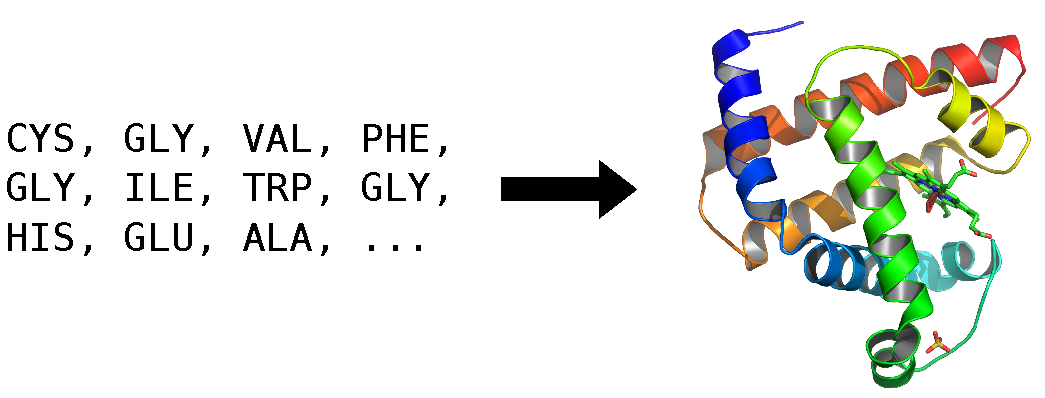
\includegraphics[width=0.7\textwidth]{psp.pdf}
    \end{center}
%   \item is a more general term than \textit{Protein Folding}, which denotes a
%     simulation of the entire folding process.
%   \item will have many applications in medicine and biotechnology.
\end{frame}

\begin{frame}[t, fragile]
  \frametitle{From C$_\alpha$-trace to an all-atom model}
  \begin{columns}
    \column{5cm}
  \begin{figure}
    \centering
    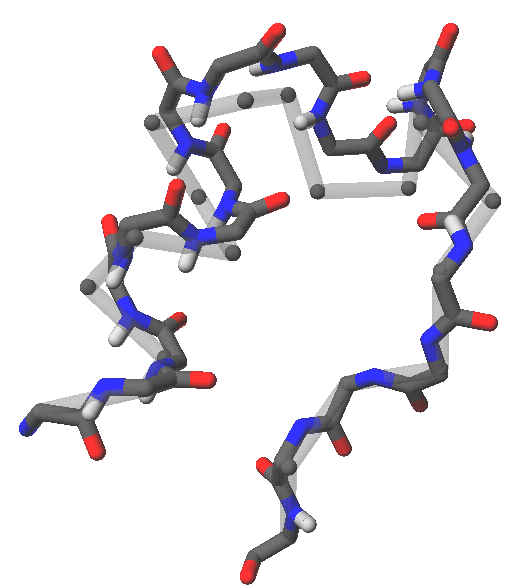
\includegraphics[width=\textwidth]{../rapport/figures/forside.png}
    \caption{Fitting of an all-atom model to a C$_\alpha$-trace}
    \label{fig:front}
  \end{figure}

  \column{5cm}

  \begin{figure}
    \centering
    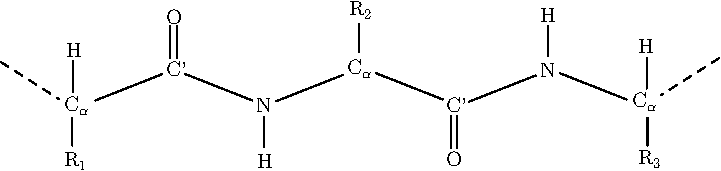
\includegraphics[width=\textwidth]{../rapport/figures/amino_connect.pdf}
    \caption{All-atom model}
    \label{fig:front}
  \end{figure}

  \begin{figure}
    \centering
    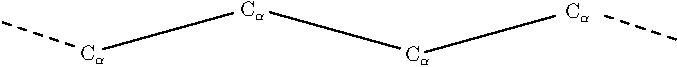
\includegraphics[width=\textwidth]{../rapport/figures/Calpha_backbone.pdf}
    \caption{C$_\alpha$-trace}
    \label{fig:front}
  \end{figure}
  \end{columns}
\end{frame}

\section{Protein geometry}
\subsection{Protein geometry}
\begin{frame}[t, fragile]
  \frametitle{Protein geometry}
  \framesubtitle{Needed measures}
  
  \vspace{0.5cm}

  \begin{figure}
    \centering
    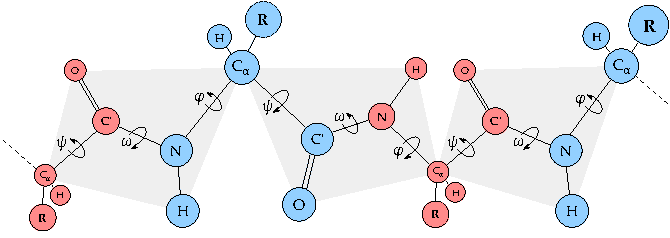
\includegraphics[width=\textwidth]{../rapport/figures/protein-torsion-angles.pdf}
    \caption{Bond angles, bond lengths and torsion angles}
    \label{fig:front}
  \end{figure}

\end{frame}

\begin{frame}[t, fragile]
  \frametitle{Protein geometry}
  \framesubtitle{Measured values}

\vspace{-0.5cm}
  \begin{columns}
 \column{5.5cm}
  \centering
\begin{table}
  \caption{Average bond lengths}
\begin{small}
  \begin{tabular}{lrr}
    \toprule
    \multicolumn{1}{c}{Bond} & \multicolumn{1}{c}{Avg. length} & \multicolumn{1}{c}{Std.dev.} \\ \midrule 
    C-O   & 1.2260 Å & 0.0188 Å\\
    CA-C  & 1.5272 Å & 0.0191 Å\\
    N-CA  & 1.4680 Å & 0.0237 Å\\
    C-N   & 1.3234 Å & 0.0215 Å\\
    N-H   & 0.9793 Å & 0.0342 Å\\
    CA-CB & 1.5327 Å & 0.0228 Å\\
    CA-HA & 1.0747 Å & 0.0307 Å\\ \bottomrule
  \end{tabular}
\end{small}
  \vspace{1mm}
  \label{tab:average_bond_lengths}
\end{table}

\column{5.5cm}
\begin{table}
  \centering
  \caption{Average bond angles}
\begin{small}
  \begin{tabular}{lrr}
    \toprule
    \multicolumn{1}{c}{Bond} & \multicolumn{1}{c}{Avg. angle} & \multicolumn{1}{c}{Std.dev.} \\ \midrule 
    H-N-CA & $118.9553^\circ$ & $1.9979^\circ$\\
    N-CA-C & $110.6099^\circ$ & $2.4668^\circ$\\
    CA-C-O & $120.7088^\circ$ & $1.3064^\circ$\\
    CA-C-N & $116.7804^\circ$ & $1.7682^\circ$\\
    C-N-CA & $121.4547^\circ$ & $1.9946^\circ$\\
    C-N-H  & $119.5112^\circ$ & $2.1599^\circ$\\ \bottomrule
  \end{tabular}
\end{small}
  \vspace{1mm}
  \label{tab:average_bond_angles}
\end{table}

\end{columns}
\end{frame}

\begin{frame}[t, fragile]
  \frametitle{Amino-acid geometry}
  \vspace{0.5cm}
  \begin{figure}
    \centering
    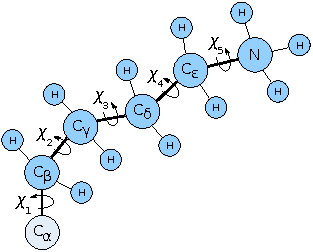
\includegraphics[width=0.5\textwidth]{../rapport/figures/lysine.pdf}
    \caption{$\chi$-angles on Lysine}
    \label{fig:front}
  \end{figure}
\end{frame}

\begin{frame}[t, fragile]
  \frametitle{RMSD as quality measure}
  
  \textbf{RMSD} is a distance measure between corresponding atoms in two structures:
\begin{displaymath}
  \label{eq:rmsd}
  \text{RMSD}(\v{A}, \v{B}) = \sqrt{\frac{1}{n}\sum_{i=1}^n |\v{a}_i - \v{b}_i|^2}
\end{displaymath}

Minimizing RMSD by translation and rotation gives an \textit{optimal
  superpositioning} of the two structures and the RMSD at this point
is called the lRMSD.\\\vspace{0.5cm}

We only include C$_\alpha$-atoms and use lRMSD as a quality measure
which we minimize by performing $\phi$ and $\psi$ rotations.

  
\end{frame}

% Anders
\section{Backbone fitting}
\subsection*{}
\begin{frame}[t, fragile]
  \frametitle{Backbone fitting} 
%  \framesubtitle{subtitle}
\begin{columns}[c]
\column{2.3in}
\\\vspace*{4mm}
\textbf{Problem:} Given an unfolded protein and a C$_\alpha$-trace, we want to restructure the protein such that the RMSD from the C$_\alpha$-trace is minimal.
\\\vspace*{4mm}
\textbf{Solution:} Inverse kinematics! Different flavors of IK algorithms exist and have been applied to protein folding.
\\\vspace*{8mm}
We use cyclic coordinate descent.
\column{2in}
	\vspace*{-3.2mm}
	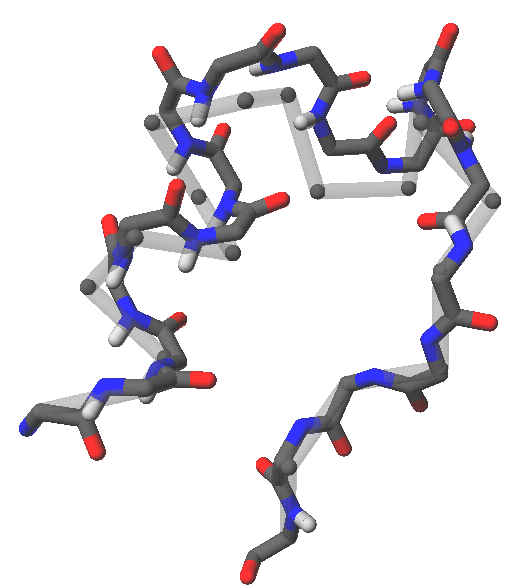
\includegraphics[width=2in]{../rapport/figures/forside.png}
\end{columns}
\end{frame}

\begin{frame}[t, fragile]
\frametitle{Backbone fitting} 
\framesubtitle{Cyclic coordinate descent}
\begin{figure}
	\centering
	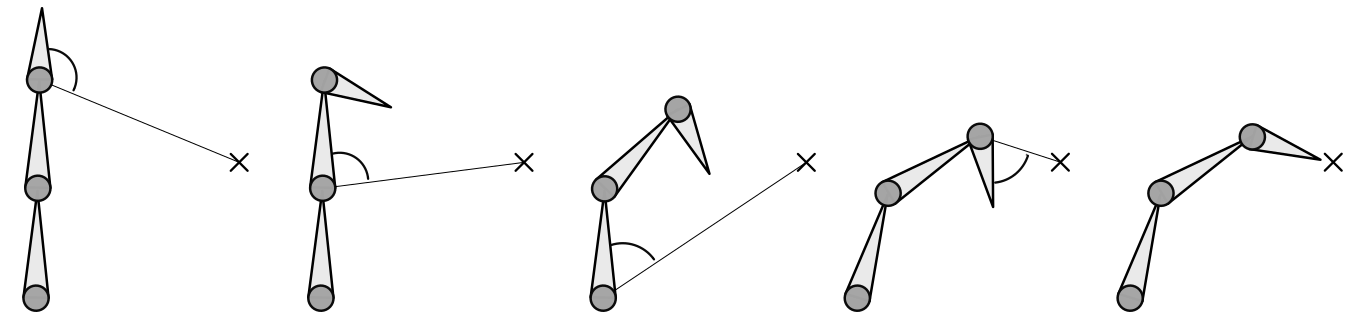
\includegraphics[width=4.3in]{ccd2d}
	\caption{Example of cyclic coordinate descent in 2D.}
\end{figure}
\vspace*{2mm}
Cyclic coordinate descent has the advantage of being fast, numerically stable, flexible and simple to implement.
\end{frame}




\begin{frame}[t, fragile]
\frametitle{Backbone fitting} 
\framesubtitle{Windowed cyclic coordinate descent}


\begin{columns}[c]
\column{2.4in}
CCD on protein backbones
\vspace*{3mm}
\begin{itemize}
\item Must use \emph{windowed} multipoint \emph{end-effector} to avoid local optimas.

\item Angles are chosen to minimize the sum of distances $S$ between C$_\alpha$ in the window.
$$\hspace*{-8mm}S=||\v{d}_1||+||\v{d}_2||+||\v{d}_3||$$

\item Folding is performed in both directions interchangeably.
%\item Folding is performed in directions.
%\item CCD is Iterates in both directions
\end{itemize}

%In 3D with a multipoint \emph{end-effector}, the CCD algorithm is more complex 
%\item 3D
%\item Multipoint \emph{end-effector}

%\vspace*{-2mm}
\hspace*{4.3cm}
\parbox{4cm}{
\begin{flushleft}
\footnotesize{
Adjusting an angle with a 
%\\\hspace*{2.8cm}
CCD window size $w=3$
}
\end{flushleft}
}

\column{2.2in}
\begin{center}
\vspace*{-6mm}
\hspace*{-4mm}
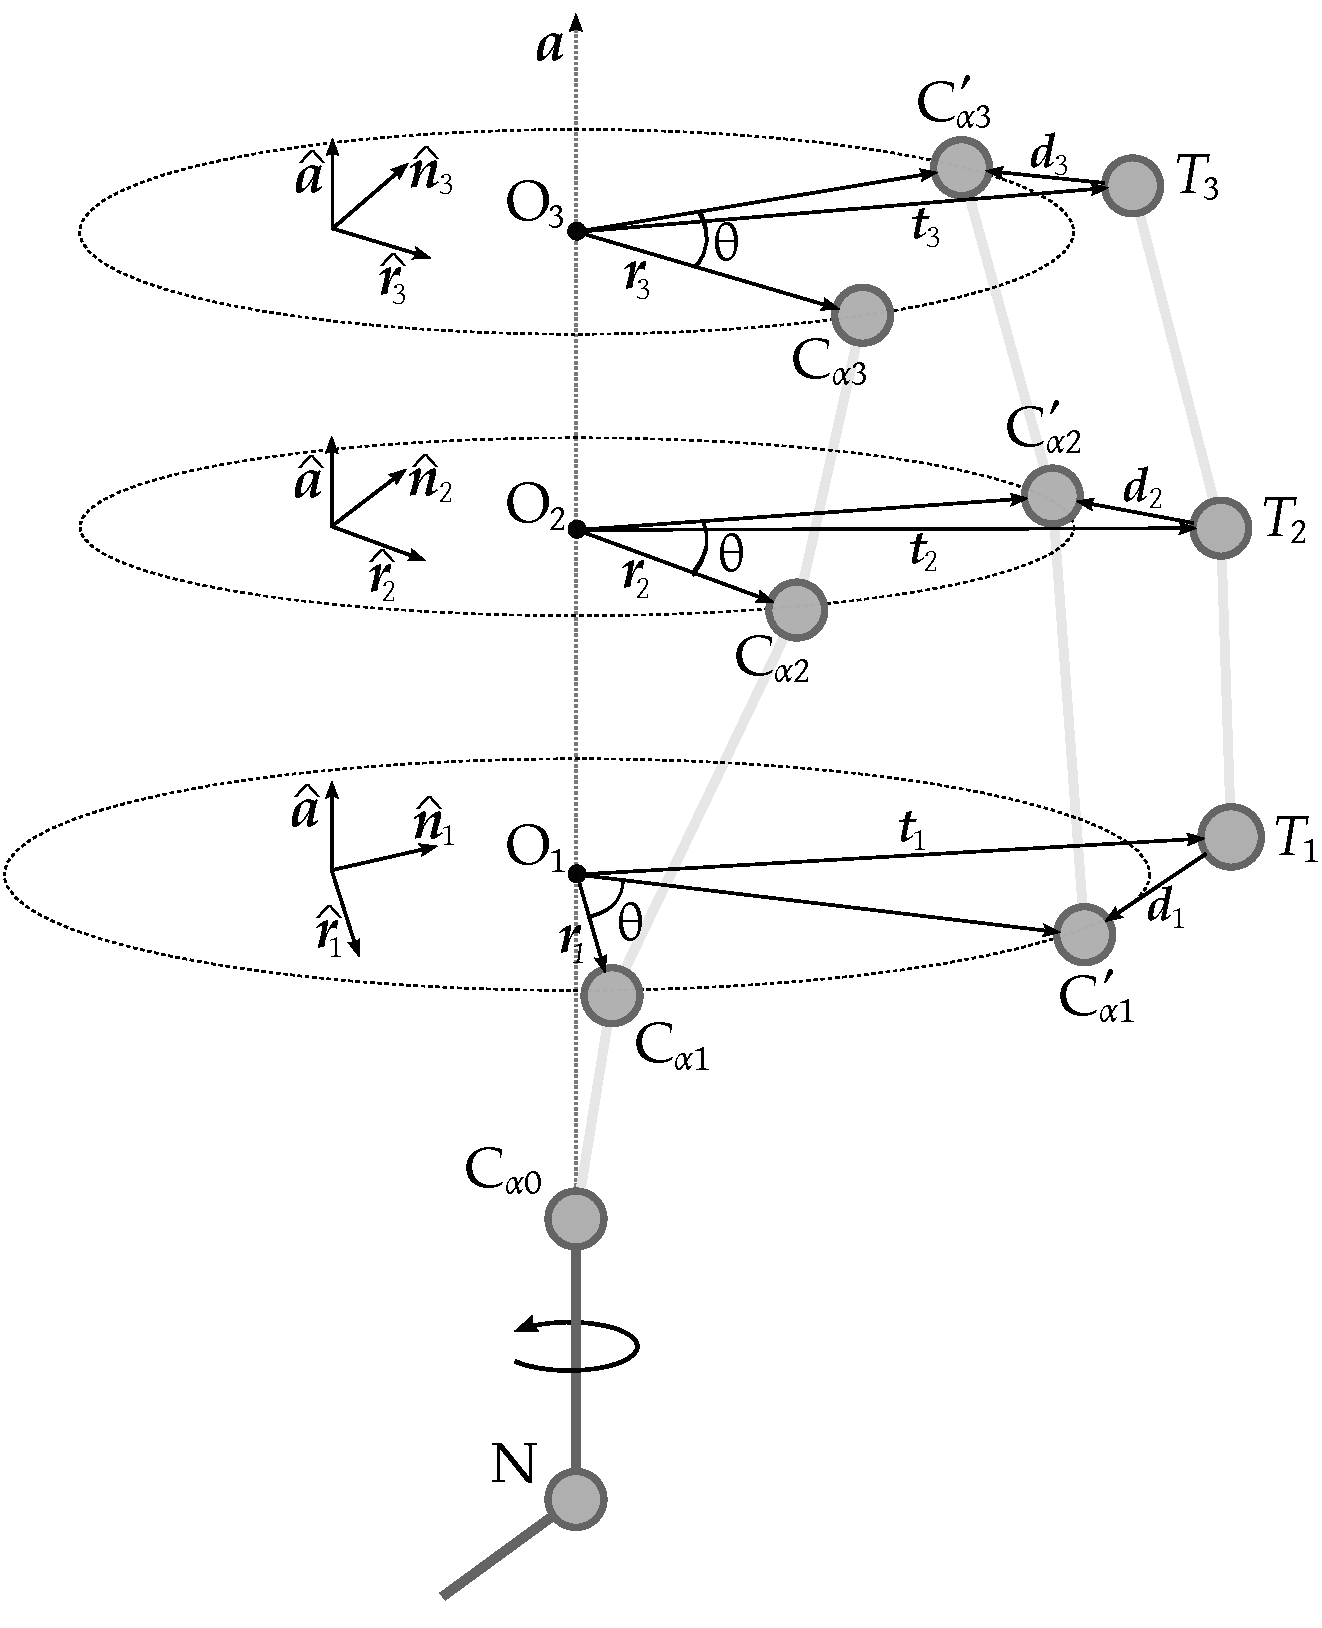
\includegraphics[width=2.3in]{ccd}
\end{center}

\end{columns}
\end{frame}

\begin{frame}[t, fragile]
\frametitle{Backbone fitting} 
\framesubtitle{Results}
\vspace*{5mm}
\begin{columns}[t]
\column{2.3in}
\centering
%Original\\
\hspace*{-3mm}
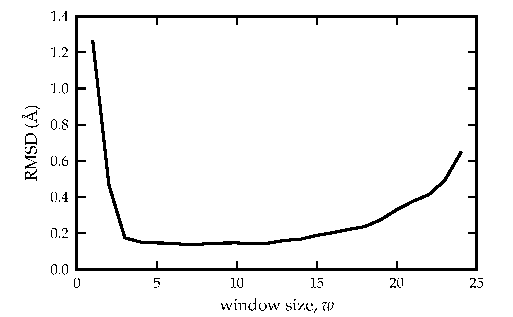
\includegraphics[width=2.5in]{plot_rmsd}\\
\small{RMSD as a function of the window size.}

\column{2.3in}
\centering
%Fitted backbone\\
\hspace*{-.4cm}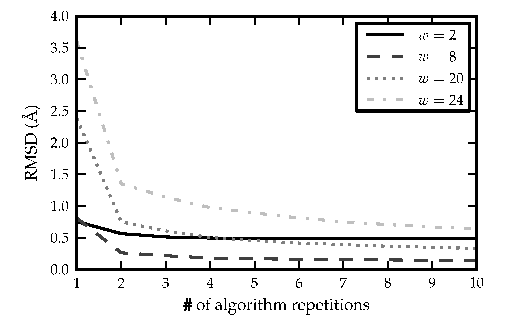
\includegraphics[width=2.5in]{plot_rmsd_convergence}\\
\small{RMSD as the fitting progresses for different
choices of window size w.}
\end{columns}
\end{frame}


\begin{frame}[t, fragile]
\frametitle{Backbone fitting} 
\framesubtitle{Results}

Ramachandran plots are somewhat similar.

\vspace*{2mm}
\begin{columns}[c]
\column{1.7in}
\centering
\begin{small}Original backbone\end{small}
\\
\hspace*{-.33cm}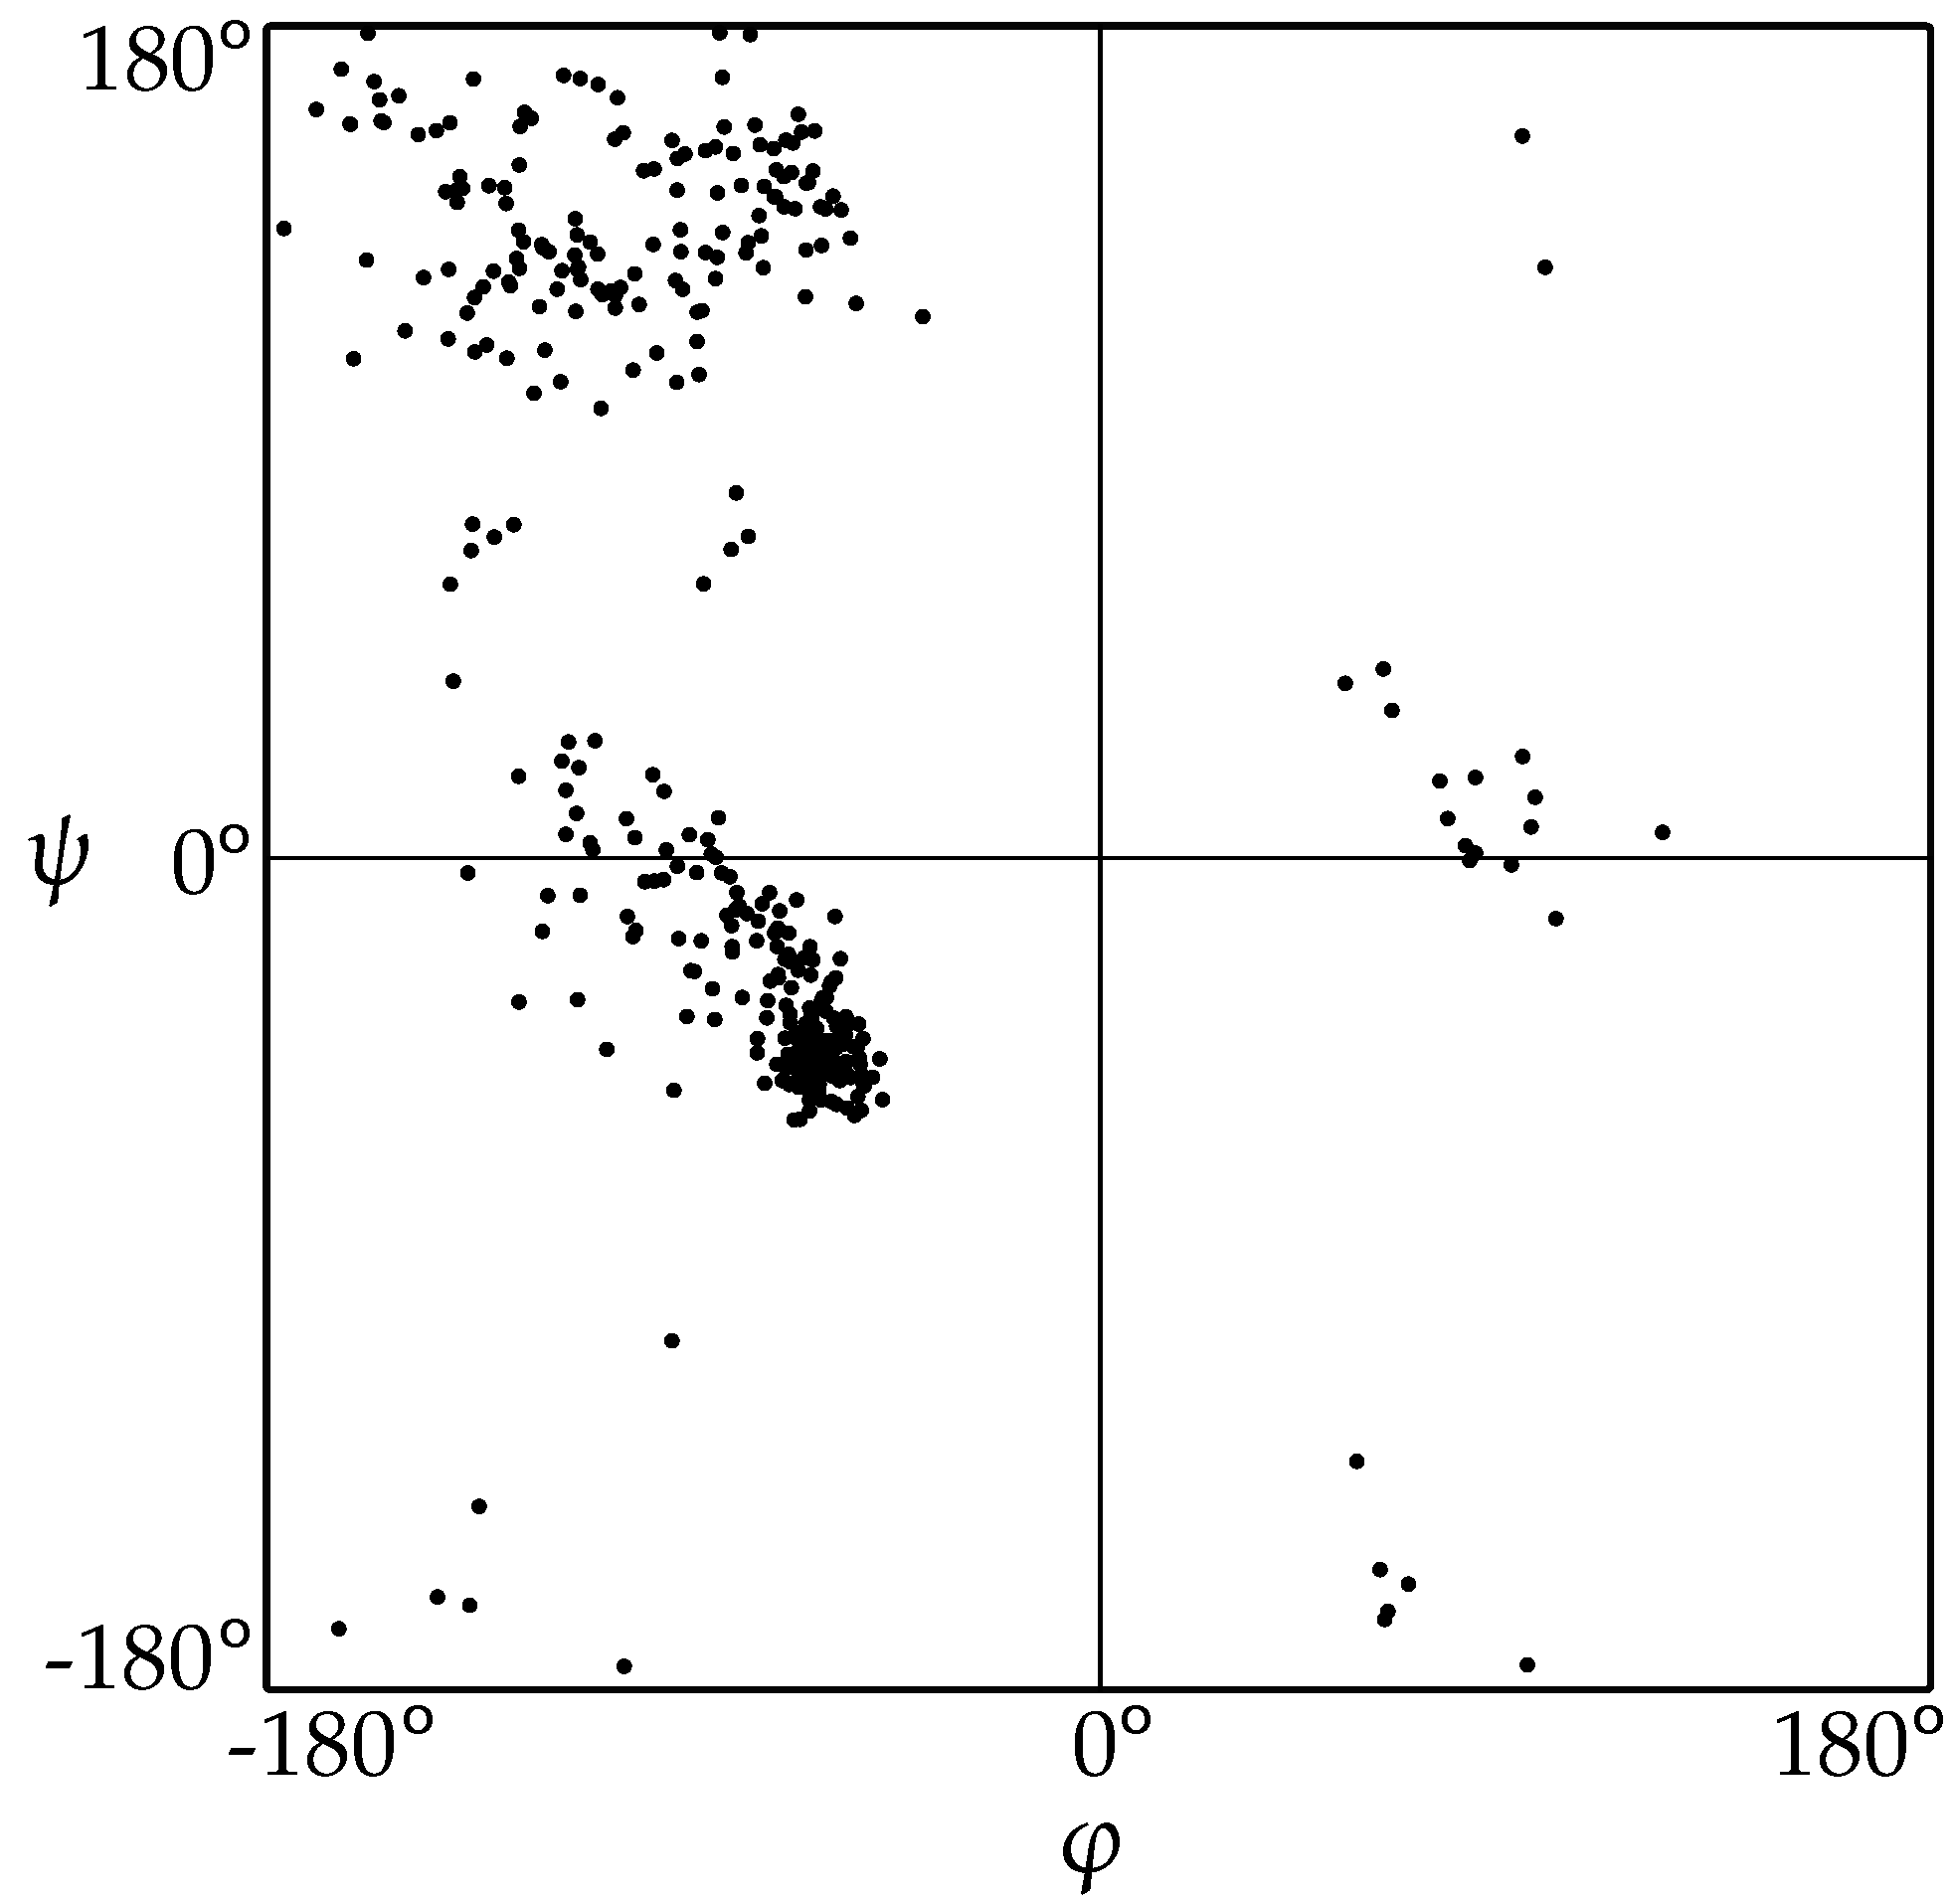
\includegraphics[width=1.7in]{plot_ramachandran_orig}

\column{1.7in}
\centering
\begin{small}Fitted backbone\end{small}
\\
\hspace*{-.4cm}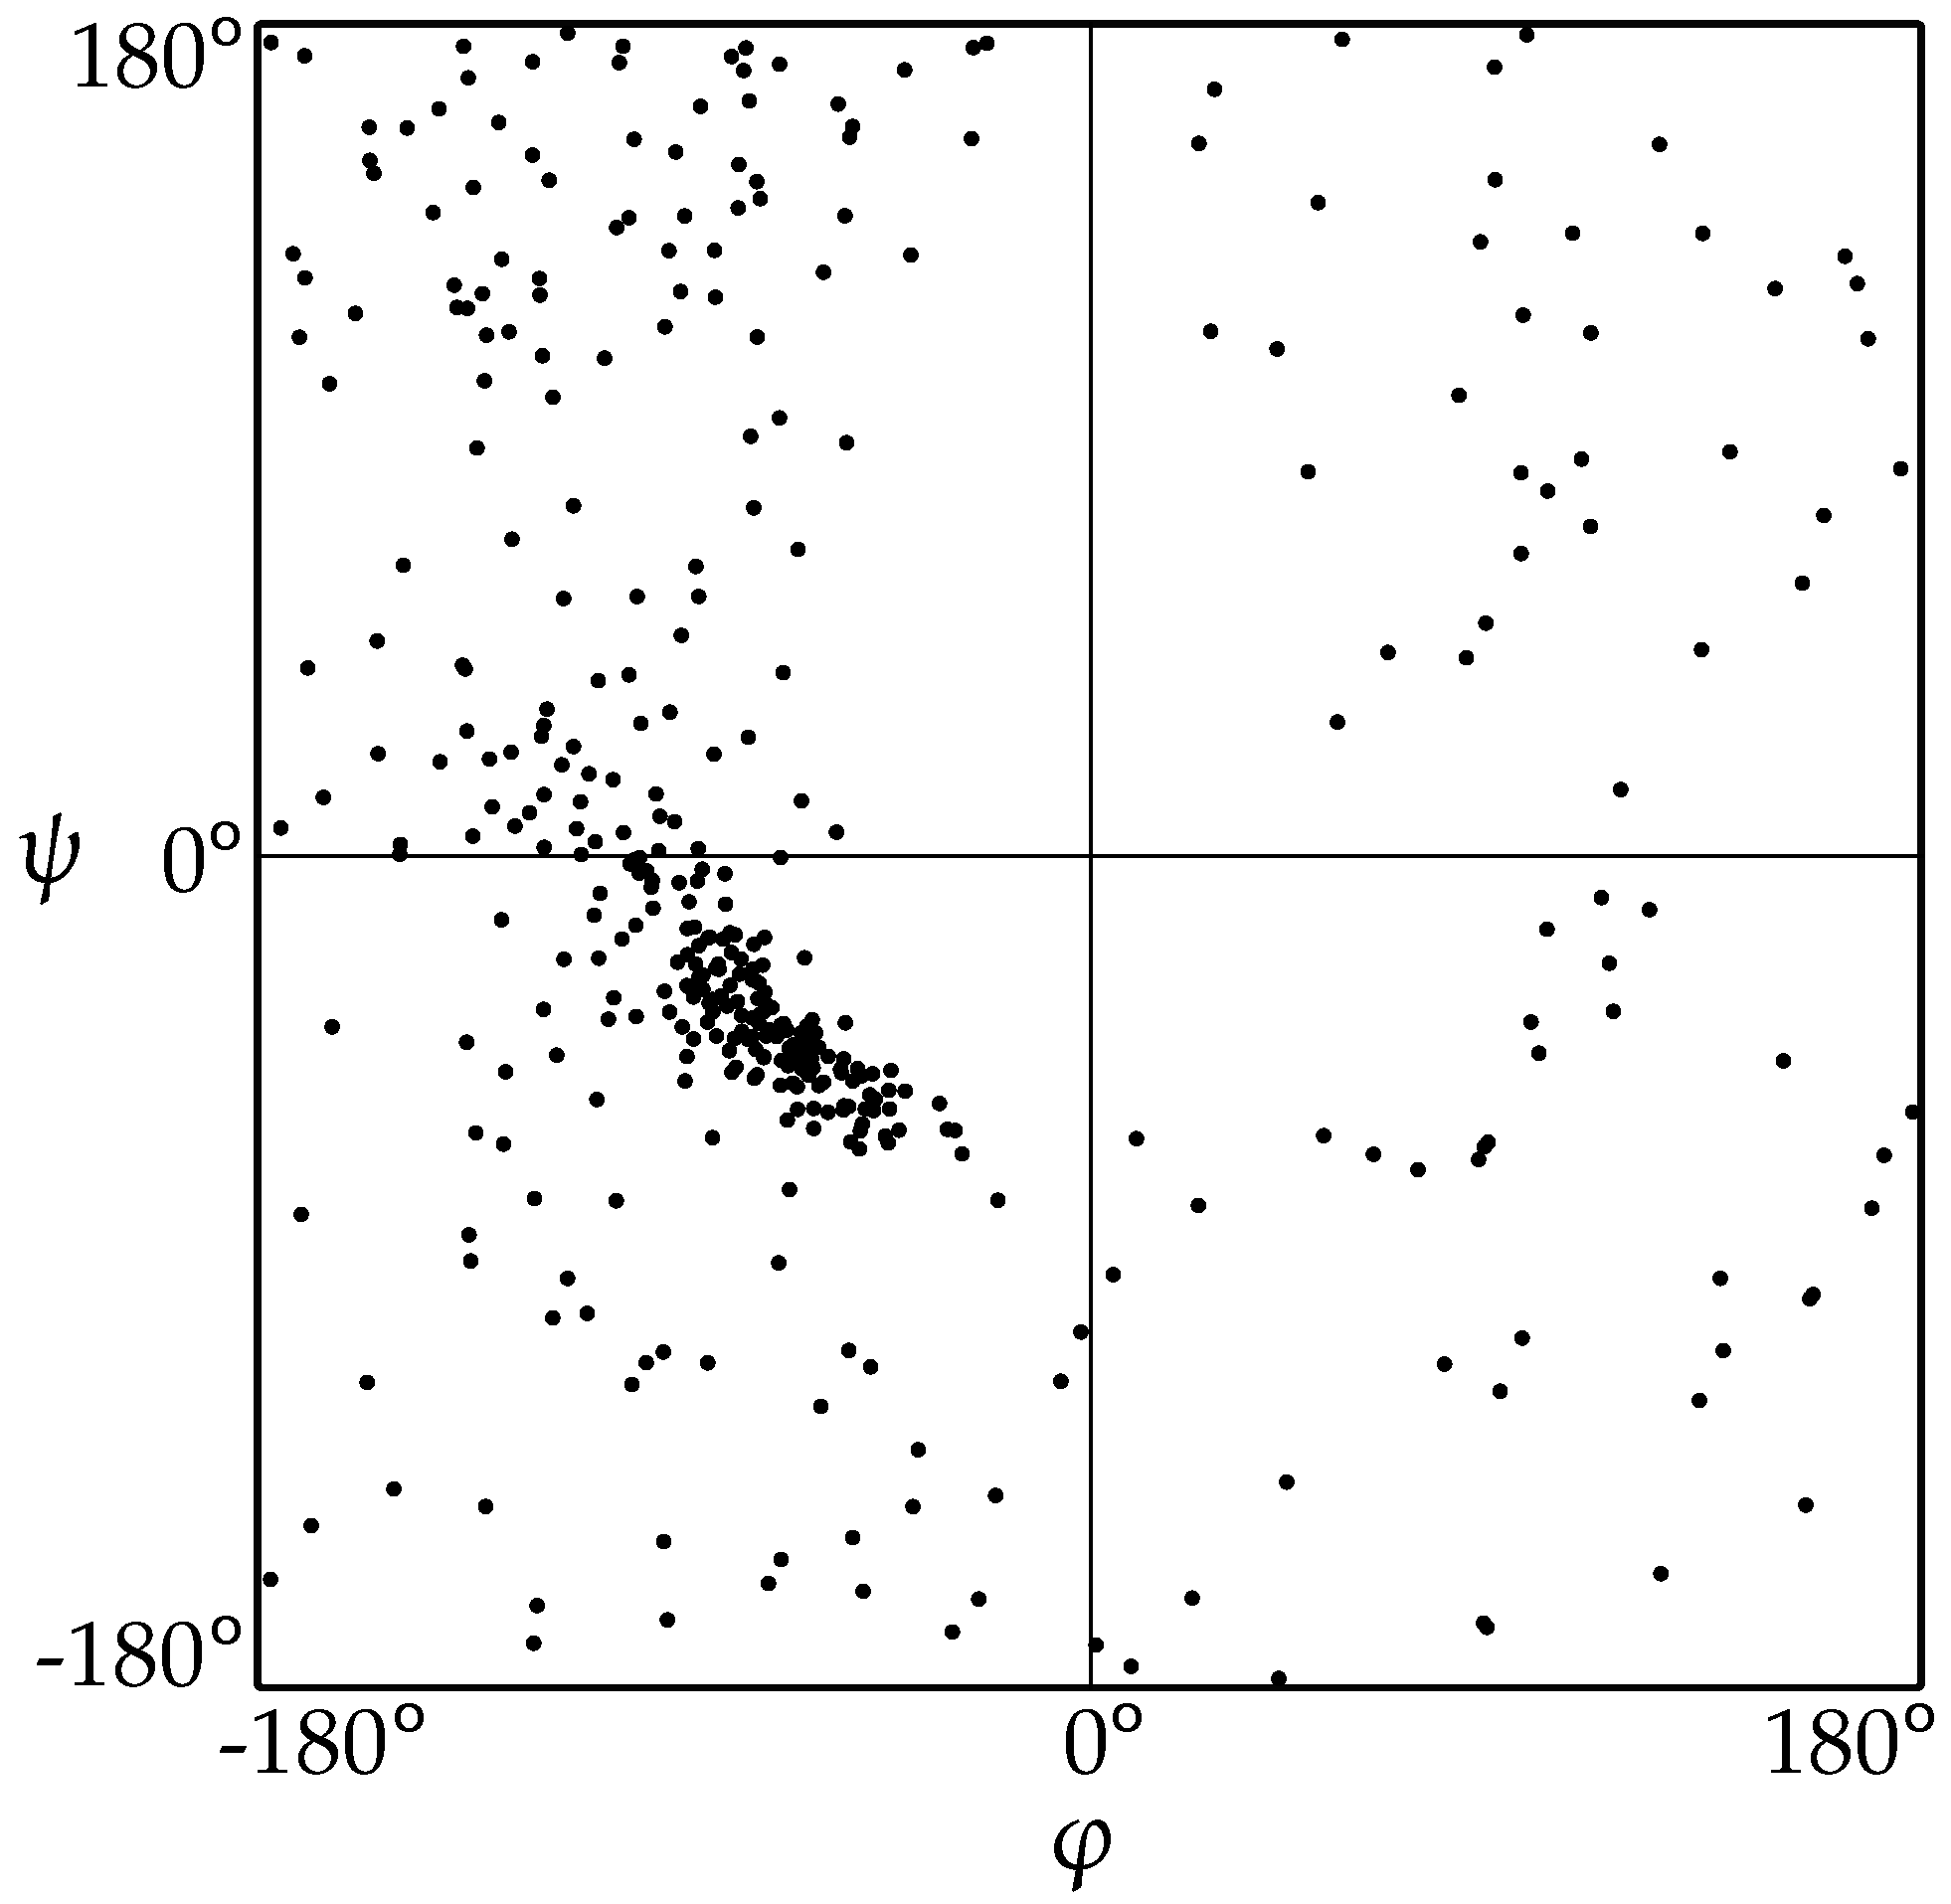
\includegraphics[width=1.7in]{plot_ramachandran}
\end{columns}
\vspace*{2mm}

More realistic Ramachandran plots can be achieved by using a probability map to accept or reject proposed sets of $\phi$ and $\psi$ angles.
%Ramachandran plot of (a) an original protein of length 415 (b) a protein backbone fitted to the original protein (RMSD = 0.15 Å).

\end{frame}



% Esben

\section{Selecting rotamers}

\subsection{dummy}
\begin{frame}
	\frametitle{Rotamers}
	
	\begin{itemize}
		\item Rotamer
		\begin{itemize}
			\item Amino acid with set of $\chi$ angles
			\item Probabilities
		\end{itemize}
		\item Dunbrack
		\begin{itemize}
			\item Open license
			\item Widely used
			\item Simple format
		\end{itemize}
	\end{itemize}
	
\end{frame}

\subsection{dummy}
\begin{frame}
	\frametitle{Collision detection}
	
	\begin{itemize}
		\item Implicit H-atoms
		\item No description in literature
		\item Fixed collision distance: 1.25 Å
		\begin{itemize}
			\item Larger distance would causes collisions in known protein structures
			\item Smaller distance would cause the structure to become sparse
		\end{itemize}
	\end{itemize}
	
\end{frame}

\subsection{dummy}
\begin{frame}
	\frametitle{Algorithm}
	\begin{columns}[c]
	\column{5.5cm}
	
	% \begin{algorithm}
	% % \caption{Overview of the general algorithm using leapfrogging}
	% \begin{algorithmic}
	% 	\FOR{each side-chain}
	% % 	% 	\STATE Reset $\chi$ angles
	% % 	% \ENDFOR
	% % 	% \FOR{each side-chain}
	% % 	% 	\FOR{each colliding side-chain}
	% % 	% 		\STATE Resolve recursively
	% % 	% 	\ENDFOR
	% 	\ENDFOR
	% \end{algorithmic}
	% \end{algorithm}
	
	% \begin{lstlisting}
	\texttt{For each side-chain}\\
	\texttt{\;\;\;\;Reset $\chi$ angles}\\
	\texttt{For each side-chain}\\
	\texttt{\;\;\;\;For each colliding side-chain}\\
	\texttt{\;\;\;\;\;\;\;\;Resolve recursively}\\
 	% \end{lstlisting}

	% For each side-chain
	% 	Reset $\chi$ angles
	% For each side-chain
	% 	For each colliding side-chain
	% 		Resolve recursively

	% \begin{itemize}
	% 	\item For each side-chain
	% 	\begin{itemize}
	% 		\item Reset $\chi$ angles
	% 	\end{itemize}
	% 	\item For each side-chain
	% 	\begin{itemize}
	% 		\item For each colliding side-chain
	% 		\begin{itemize}
	% 			\item Resolve recursively
	% 		\end{itemize}
	% 	\end{itemize}
	% \end{itemize}
	
% \end{frame}

% \begin{frame}
	% \frametitle{Algorithm}
	
	\column{5cm}
	\begin{figure}
		% \centering
		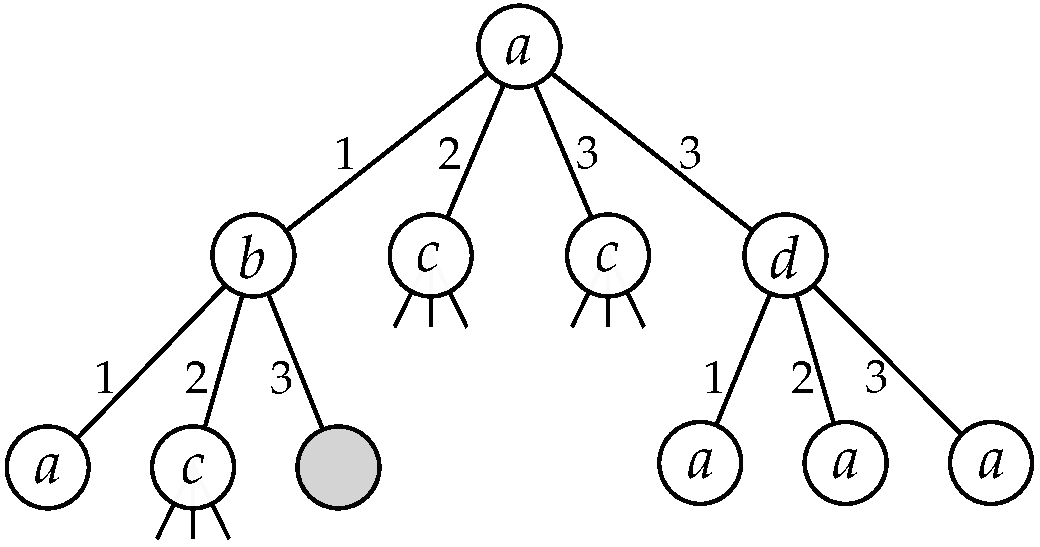
\includegraphics[width=5cm]{../rapport/figures/rotamersearch.pdf}
	\end{figure}
	
	\end{columns}
\end{frame}

\subsection{dummy}
\begin{frame}
	\frametitle{Performance}
	
	\begin{itemize}
		\item Backbone fitting quality affects side-chain collisions
		\item Fitting resolves $4/5$ collisions
		\item Some collisions can not be solved
		\begin{itemize}
			\item Proline collides with backbone
			\item Side-chains are placed too close to each other
		\end{itemize}
		\item Search depth of 3 seems optimal
	\end{itemize}
	
\end{frame}

\subsection{dummy}
\begin{frame}
	\frametitle{Performance}
	
	\begin{figure}
		\centering
		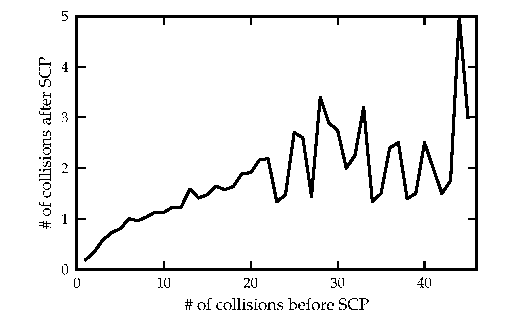
\includegraphics[width=.75\columnwidth]{../rapport/figures/plot_scp}
	\end{figure}
	
\end{frame}


\section{Conclusion}

\subsection{dummy}
\begin{frame}
	\frametitle{Conclusion and Future Work}
    \begin{itemize}
    \item We have derived our own variant of the CCD method for the
      problem of fitting our all-atom model to the C$_\alpha$-trace.
    \item We typically reach a RMSD of less than 0.2 Å.
    \item We successfully decomposed the problem into two separate
      tasks. It could be interesting to adjust the backbone according
      to side-chain collisions.
    \item To avoid collisions caused by illegal $\phi$ and $\psi$
      angles, it could be investigated
      how to integrate Ramachandran propability maps.
    \end{itemize}
\end{frame}


\end{document}
